%导言区
\documentclass[12pt]{ctexart}
\title{\heiti \LaTeX 笔记}
\author{\kaishu zcz}
\date{\today}

%**************************包的引用**********************************
% 页面设置
\usepackage{fancyhdr}        % 页脚页眉
\usepackage{lastpage}        % 获取总共的页数
\usepackage{geometry}        % 设置页边距
% 数学环境
\usepackage{amsmath}
\usepackage{amssymb}
% 矩阵斜省略号iddots
\usepackage{mathdots}
% 插入图片
\usepackage{graphicx} 		%插入图片的宏包
\usepackage{float} 			%设置图片浮动位置的宏包(图片参数为H时必须)
\graphicspath{{./figure/}}  %搜索路径
% 多图排版
\usepackage{subfigure} 		%插入多图时用子图显示的宏包
% 三线表宏包
\usepackage{booktabs}

%**********************************全文格式设置**********************
% 设置纸张为A4,上下边距为3.2、2.8cm,左右边距为2.5cm 
\geometry{a4paper,left=2.5cm,right=2.5cm,top=3.2cm,bottom=2.8cm}
% 各级标题格式的设置
\setcounter{tocdepth}{4}     % 设置目录显示的深度为4
\setcounter{secnumdepth}{4}  % 设置章节显示的深度为4
\ctexset{
	section={
		format=\zihao{-3} \heiti \centering,
		name = {第,章},
		% number = \chinese{section},
		beforeskip=30pt,
		afterskip=30pt
	},
	subsection={
		format = \zihao{-3} \heiti \raggedright,
		beforeskip=18pt,
		afterskip=12pt
	},
	subsubsection={
		format=\fontsize{13pt}{20pt} \heiti \raggedright,
		beforeskip=12pt,
		afterskip=12pt,
	},
	paragraph={
		format=\zihao{-4} \heiti \raggedright,
		beforeskip=6pt,
		afterskip=6pt,
	}
}
%设置页脚页眉
\pagestyle{fancy}                            % 使用fancy风格
%\fancyhf{}                                   % 清除所有的页眉页脚
%\renewcommand\headrulewidth{0pt}             % 去除页眉横线
\fancyhead[L]{\heiti \LaTeX 笔记}
\fancyfoot[C]{\kaishu{第 \thepage 页,共 \pageref{LastPage} 页}}   
% 页脚中,第x页,共x页
% \renewcommand{\baselinestretch}{1.5}          % 全文设置1.5倍间距
\setlength{\baselineskip}{20pt}                 % 全文设置1.5倍间距
% 设置参考文献的数字为右上角
\newcommand{\supercite}[1]{\textsuperscript{\cite{#1}}}
%************************************正文创作************************


%************************************正文区**************************
\begin{document}
	
%设置标题
\maketitle
%设置页眉页脚
\thispagestyle{empty}
\tableofcontents
\newpage
\setcounter{page}{1}


%*****************************摘要*******************************%
\begin{abstract}
	
\setlength	%\parindent{1em}	%设置缩进
1.文档类型及章节设置:
\par article普通文章,book,report,beamer幻灯片,letter
\par 中文文档类型:ctexart,ctexbook,ctexrep
\par 正文可设置章节section,子章节subsection,次级子章节subsubsection。
如果文档类型是ctexbook,还可以添加part(部分)和chapter(章)。\\

2.空格及缩进\par
一个换行符空 \ 格,
{\ quad空格},\ setlength设置缩进,\ noindent取消缩进\\

3.换行(缩进or不缩进):\par
{$\backslash$ par换行缩进}

{空行换行缩进}
~\\ 
{~ $\backslash$ $\backslash$换行不缩进\\}

4.反斜杠\&括号的美化输出\&星号:\par
textbackslash文本模式反斜杠,backslash数学模式反斜杠

$(\frac{1}{2})$,$\left ( \frac{1}{2} \right )$,$\ast$,*

\end{abstract}
\newpage


%*****************************第一章*******************************
\section{预备}

%列表
\subsection{列表}
\par 无序列表
\begin{itemize}
	\item 列表项	
	\item 列表项
\end{itemize}
\par 有序列表
\begin{enumerate}
	\item 列表项	
	\item 列表项
\end{enumerate}

%图片
\subsection{图片}
图的标题放在图的下方.

\begin{figure}[H]	%H为当前位置,htbp为浮动图形(美观考虑)
	\centering
	
\includegraphics[width=0.4\textwidth]{图片1.jpg}
	% 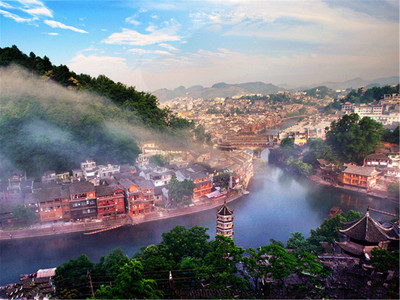
\includegraphics[width=8cm]{1.png}
	\caption{单图排版}
	\label{t1}
\end{figure}

\begin{figure}[H]	%H为当前位置,htbp为浮动图形(美观考虑)
	\subfigure{
		\begin{minipage}{0.5\textwidth}
			\centering
			
\includegraphics[width=0.9\textwidth]{图片1.jpg}
		\end{minipage}
	}
	\subfigure{
		\begin{minipage}{0.5\textwidth}
			\centering
			
\includegraphics[width=0.9\textwidth]{图片1.jpg}
		\end{minipage}
	}
	\caption{多图排版}
	\label{t2}
\end{figure}

\subsection{交叉引用}
如图\ref{t1},如表\ref{b1}

%表格
\subsection{表格}

\begin{table}[H]
\centering
\caption{表格}
	\begin{tabular}{|p{2cm}|c|c|}
		\hline
		单元格1&单元格2&单元格3\\
		\hline\hline
		单元格4&单元格5&单元格6\\
		\hline
		单元格7&单元格8&单元格9\\
		\hline
	\end{tabular}\label{b1}
\end{table}

%三线表
\begin{table}[H]
	\centering
	\caption{三线表}
	\begin{tabular}{cc}
		\toprule[1.5pt]
		\makebox[0.3\textwidth][c]{符号}	&  \makebox[0.4\textwidth][c]{意义} \\
		\midrule[1pt]
		$ W $	    	& 某一小时内该路段运行总收益-总成本   \\ 
		$ W_0 $	    	& 区分高峰和低峰的一个临界值  \\ 
		$ P $	    	& 线路在一小时内所有站的总上车人数 \\ 
		$ x $	    	& 线路在一小时内的车辆数 \\  
		$ T_t $	    	& 长期趋势项 \\ 
		$ M_t $	    	& 简单移动平均项 \\ 
		\bottomrule[1.5pt]
	\end{tabular}\label{b2}
\end{table}

%newcommand
\subsection{定义新命令}
%newcommand用于定义新命令,\circ——{。}
\newcommand\degree{^\circ}
勾股定理:设直角三角形 $ABC$,其中 $\angle C=90 \degree$,则有:
$$AB^2=BC^2+AC^2$$

%帮助文档
\subsection{帮助文档}
texdoc ctex:ctex宏包手册{\par}
texdoc lshort-zh:一份不太简短的{\LaTeX}介绍


%********************************第二章******************************
\section{字体设置}
\subsection{字体设置}

\noindent

1.分类
\par 字体共5种属性:编码(正文字体编码,数字字体编码),族(罗马,无衬线,打字机),
系列(粗细,宽度),形状(直立,斜体,伪斜体,小型大写),大小 \\\\

2.字体族
\par \textrm{罗马} \textsf{无衬线} \texttt{打字机} %命令
{\rmfamily 罗马} {\sffamily 无衬线} {\ttfamily 打字机} \\\\ %声明

3.字体系列
\par \textmd{Medium} \textbf{加粗}
{\mdseries Medium} {\bfseries 加粗} \\\\

4.字体形状
\par \textup{直立} \textit{斜体} \textsl{伪斜体} \textsc{小型大写}
{\upshape 直立} {\itshape 斜体}
{\slshape 伪斜体} {\scshape 小型大写} \\\\

5.中文字体
\par {\songti 宋体} \quad {\heiti 黑体} \quad {\fangsong 仿宋}
\quad {\kaishu 楷书}\\\\
%对于中文:粗体\textbf{粗体=黑体},斜体\textit{斜体=楷书}

6.字体大小
\par {\tiny Hello!} {\small Hello!} {\normalsize Hello!} 
{\large Hello!} {\huge Hello!} 

%文档类型的大小参数设置:10pt,11pt,12pt
%中文字号大小设置
\zihao{5} 你好!
\newcommand\myfont{\textbf{\textsf 你好!}}\myfont \\\\

\subsection{字体大小}
1.全局模式: 

documentclass[12pt]{article}

2.局部模式: \\
Hello Latex.\\
\tiny Hello Latex.\\
\scriptsize Hello Latex.\\
\footnotesize Hello Latex.\\
\small Hello Latex.\\
\normalsize Hello Latex.\\
\large Hello Latex.\\
\Large Hello Latex.\\
{\LARGE Hello Latex.}\\
\begin{huge} 
	Hello Latex. 
\end{huge}
\normalsize		%恢复全局字体


%********************************第三章******************************
\section{快捷键}

\subsection{“Idefix”and“查看”}
\begin{itemize}
	\item 注释:	Ctrl+T	
	\item 取消注释: Ctrl+U	
	\item 替换:	Ctrl+R
	\item 查找:	Ctrl+F
	\item 粘贴为LaTeX:Ctrl+Shift+V
	\item 转到定义:Ctrl+Alt+F
	\item 全屏模式:F11+Fn
\end{itemize}

\subsection{“LaTeX”}
\begin{itemize}
	\item 项目:Ctrl+Shift+I	
	\item 斜体:Ctrl+I
	\item 粗体:Ctrl+B
	\item 打字机:Ctrl+Shift+T
	\item 小型大写字母:Ctrl+Shift+C
	\item 重点:Ctrl+Shift+E
	\item 新行:Ctrl+Enter	
	\item 开始{环境}:Ctrl+E
	\item 插入对下一个标签的引用:Ctrl+Alt+R
\end{itemize}

\subsection{“数学”}
\begin{itemize}
	\item 内联数学模式:Ctrl+Shift+M
	\item 显示数学模式:Alt+Shift+M
	\item 编号方程:Ctrl+Shift+N
	\item 下标:Ctrl+Shift+D
	\item 上标:Ctrl+Shift+U
	\item 分数:Alt+Shift+F 
	\item 平方根:Ctrl+Shift+Q
	\item 右:Ctrl+Shift+R 
\end{itemize}


%********************************第四章******************************
\section{数学公式编辑}

\subsection{行内、行间及跨行公式的表示方法}
\subsubsection{行内公式的三种表示方法}
\( a+b=b+a \)

$ a+b=b+a $

\begin{math}
	a+b=b+a\\
	\text{注意:在math环境中使用文字需要使用text指令.}
\end{math}

\subsubsection{行间公式的三种表示方法}
\[ a+b=b+a \]
$$ a+b=b+a $$
\begin{displaymath}
	a+b=b+a\\
\end{displaymath}

\subsubsection{自动编号公式}
\begin{equation}
	a+b=b+a
\end{equation}
\begin{equation*}
	a+b=b+a
	\label{s1}
\end{equation*}
交换律如上式\ref{s1}


\subsection{多行公式:}
\subsubsection{gather环境}
\begin{gather}
	a+b=b+a	\\
	1+2=2+1	\notag \\
	E=mc^2
\end{gather}

\subsubsection{align环境}
align环境按\&符号对齐
\begin{align}
	a+b &= b+a & xy       &= 3z\\
	1+2 &= 2+1 & x \div y &= 3z\notag \\
	E   &= mc^2
\end{align}

\subsubsection{split环境}
split环境用于连等号.\par
split需要配合equation使用.\par
\begin{equation}
	\begin{split}
		\cos 2x &= \cos^2 x - \sin^2 x	\\
		&= 2\cos^2 x - 1
	\end{split}
\end{equation}


\subsection{大括号公式:}
\subsubsection{aligned环境:}
\par 第一种
$$	
f(x)=\left\{
\begin{aligned}
	x & = & \cos(t) \\
	y & = & \sin(t) \\
	z & = & \frac xy
\end{aligned}
\right.
$$
\subsubsection{array环境:}
\par 第二种
$$ F^{HLLC}=\left\{
\begin{array}{rcl}
	F_L       &      & {0      <      S_L}\\
	F^*_L     &      & {S_L \leq 0 < S_M}\\
	F^*_R     &      & {S_M \leq 0 < S_R}\\
	F_R       &      & {S_R \leq 0}
\end{array} \right. $$
\subsubsection{cases环境}
\par 第三种
cases用于分段函数,适用同时表示值和条件的情形.\par
cases需要配合equation使用.\par
$A \backslash B$更紧凑\quad
$A \setminus B$
\begin{equation}
	F(x) =
	\begin{cases}
		1,& \text{如果} x \in \mathbb{Q};	\\
		0,& \text{如果} x \in \mathbb{R} \setminus \mathbb{Q};	
	\end{cases}
\end{equation}


\subsection{希腊字母、数学函数及不等号}
\subsubsection{希腊字母}
Latex中编辑数学符号和函数,可以先打$\backslash$\,自动补全的同时也会自动纠错.

$\alpha$
$\beta$
\par
$\gamma$ \ $\Gamma$
\par
$\epsilon$
$\pi$
\par
$\omega$ \ $\Omega$

\subsubsection{数学函数}
基本函数写法
$\log$ \quad $\ln$ \quad $\sin$ \quad $\arcsin$

三角恒等式
$(sinx)^2+(cosx)^2=1$ \quad $sin^{2}x+cos^{2}x=1$

根式
$\sqrt{x+1}$ \quad $\sqrt[4]{x^2+3x}$

分式
\begin{itemize}
	\item 直接使用分式\quad {a/b}
	\item 使用frac指令\quad $\frac{a}{b}$
\end{itemize}

\subsubsection{大于等于号、小于等于号 :}
\par 简单写法 \quad $ \le \leq \ge \geq $ \\
\par 标准写法 \quad 
$\leqslant \geqslant$
$\neq$


%********************************第五章******************************
\section{矩阵}
\subsection{各种简单矩阵:}
$$
\begin{gathered}
	\begin{matrix} 0 & 1 \\ 1 & 0 \end{matrix}
	\qquad
	\begin{pmatrix} 0 & -i \\ i & 0 \end{pmatrix}
	\qquad
	\begin{bmatrix} 0 & -1 \\ 1 & 0 \end{bmatrix}
	\qquad
	\begin{Bmatrix} 1 & 0 \\ 0 & -1 \end{Bmatrix}
	\qquad
	\begin{vmatrix} a & b \\ c & d \end{vmatrix}
	\qquad
	\begin{Vmatrix} i & 0 \\ 0 & -i \end{Vmatrix}
\end{gathered}
$$
\[
\begin{pmatrix}
	a_{11} & a_{12} & \dots & a_{1n} \\
	a_{21} & a_{22} & \dots & a_{2n} \\
	\vdots  & \vdots & \ddots & \vdots \\
	1 & 1 & 1 & 1
\end{pmatrix}_{n \times n}
\]

如果要用$\iddots$,需要导入mathdots包.


\subsection{其他矩阵形式:}
\subsubsection{分块矩阵:}
\[
\begin{pmatrix}
	\begin{matrix} 0 & 1 \\ 1 & 0 \end{matrix} & \text{\Large 0}\\
	\text{\Large 0} & \begin{matrix} 0 & 1 \\ 1 & 0 \end{matrix}
\end{pmatrix}
\]

\subsubsection{三角矩阵:}
\[
\begin{pmatrix}
	a_{11} & a_{12} & \dots & a_{1n} \\
	& a_{22} & \dots & a_{2n} \\
	& & \ddots & \vdots \\
	\multicolumn{2}{c}{\raisebox{1.3ex}[0pt]{\Huge 0}}& & a_{nn}
\end{pmatrix}
\]

\subsubsection{跨列省略号:}
hdotsfor{列数}
\[
\begin{pmatrix}
	a_{11} & a_{12} & \dots & a_{1n} \\
	a_{21} & a_{22} & \dots & a_{2n} \\
	\hdotsfor{4} \\
	1 & 1 & 1 & 1
\end{pmatrix}
\]

\subsubsection{行内小矩阵:}
\begin{math}
	\left(	%手动左括号
	\begin{smallmatrix}
		x & -y \\
		y & x
	\end{smallmatrix}
	\right)	%手动右括号
\end{math}

\subsubsection{模拟赛3:}

$$min f=\sum_{i=1}^{5}w_{i1}q_{i1}+\sum_{i=1}^{5}w_{i2}q_{i2}+w_3q_3+w_4q_4+w_5q_5$$

$$s.t.\left\{
\begin{array}{rcl}
	       e_1\leq 2 &    &\text{四驱车连续不超过两辆}\\
	5 \leq d_1\leq 9 &    &\text{四驱车间隔5到9辆可以接受}\\
	       e_2\leq 2 &    &\text{柴油车连续不超过两辆}\\
	5 \leq d_2\leq 9 &    &\text{柴油车间隔5到9辆可以接受}\\
\end{array} 
\right.$$

\begin{center}
	\begin{tabular}{cc}
		\toprule[1.5pt]
		\makebox[0.3\textwidth][c]{符号}	&  \makebox[0.4\textwidth][c]{意义} \\
		\midrule[1pt]	
		$ A,B,C,D,E,F    $ &品牌,配置,动力,驱动,颜色,生产线\\
		$ A(A=1,2)       $ &品牌(A1,A2)\\
		$ B(B=1,2,...,6)  $ &配置(B1,B2,B3,B4,B5,B6)\\
		$ S $	&需求矩阵\\ 
		\bottomrule[1.5pt]
	\end{tabular}
\end{center}

\end{document}
